\section{Graphische Programmierung}
\label{sec:graphischeprogrammierung}

Trotz der einfachen Lesbarkeit der JSON-Datei, verliert man bei immer größer
werdenden Automaten leicht den Überblick und der Vorteil der Trennung von Logik
und Programmierung geht verloren. Um dieses Problem zu beheben setzen wir das
Programm „UMLet“ ein. Es ist ein freies Open-Source UML-Tool, welches mehrere
Diagramm-Arten unterstützt, unter anderem State-Charts. Gespeichert werden
diese Diagramme im xml-Format, welches wir mit dem Programm „xml2json“ (Quelle)
in eine JSON-Datei, für die weitere Verwendung, umwandeln.
%%%%%%
\subsection{UMLet - Das Programm}
\begin{figure}[ht]
\centering 
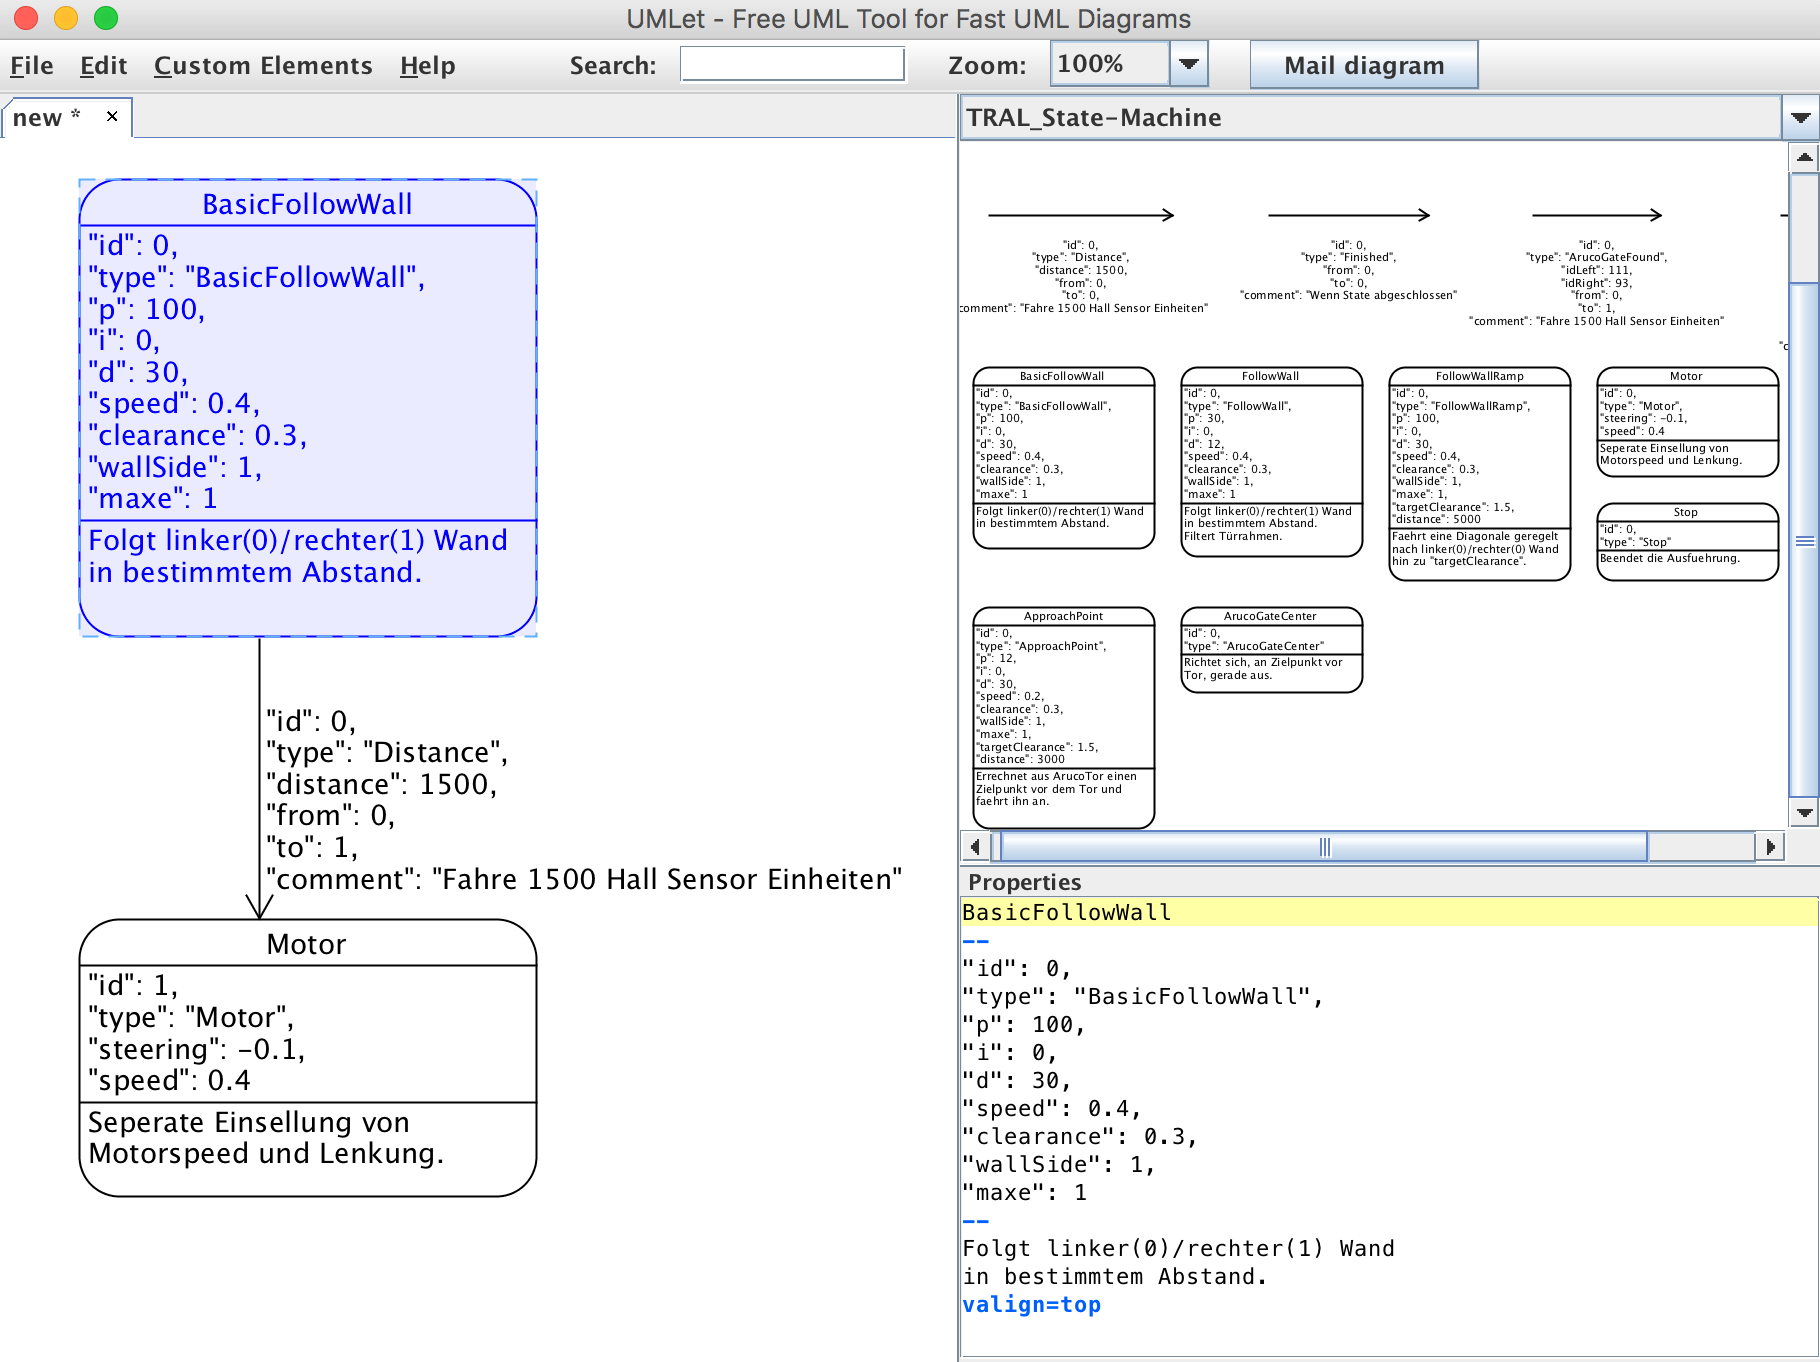
\includegraphics[width=0.90\textwidth]{images/umlet-bsp.png} 
\caption{UMLet Oberfläche}
\label{fig:umlet}
\end{figure}

Das Programm UMLet besteht aus drei Teilbereichen. Im linken Teil, dem
Arbeitsbereich, wird der eigentliche Automat erstellt. Hierfür können, schon
vordefinierte, Zustände und Transitionen aus der Vorlage „TRAL-State-Machine“
oben rechts in den Arbeitsbereich gezogen und entsprechend den eigenen Wünschen
miteinander verbunden werden. Die Vorlagen-Datei „TRAL-State-Machine.uxf“ muss
hierfür im innerhalb des Programmordners unter „../palettes“ hinterlegt sein.
Sie kann natürlich ebenfalls von dort geöffnet und gegebenenfalls erweitert
werden.
Der wichtigste Bereich ist das Fenster für die Eigenschaften jedes Zustandes
und jeder Transition unten rechts in der Ecke.
Bei Zuständen werden zwischen den beiden horizontalen Trennlinien, bei
Transitionen direkt unter dem stilisierten Pfeil (lt=->), alle Parameter
angegeben, die zur späteren Erstellungen der Objekte benötigt werden. Diese
Liste muss stets vollständig sein. Sie ist durch unsere konkrete
Implementierung im Quellcode vorgegeben und lässt sich in unserer Dokumentation
am Ende dieses Dokumentes nachlesen.
Wichtig hierbei ist noch den Zuständen und Transitionen eindeutige „IDs“ zu
vergeben, da diese grundlegend für den logischen Fluss sind.


%%%%%%
\subsubsection{uxf-Datei in JSON-Format umwandeln}
Die uxf-Dateien, welche von UMLet erstellt werden, sind intern im xml-Format
gespeichert. Sofern man das Tool „xml2json“ bereits heruntergeladen und
kompiliert hat, lassen sich diese Dateien mittels des einfachen Befehls
"\textit{./xml2json automat.uxf >> automat.json}" in eine JSON-Datei umwandeln.
Da man mittels des Aufrufs „xyz“ unseren FSM-Node starten kann und ihm diese
JSON-Datei übergeben muss, lässt sich dieser ganze Abschnitt leicht mit einem
Shell-Skript zum Umwandeln und Starten der FSM realisieren.
(skript?!)


%%%%%%
\subsubsection{Einlesen einer JSON-Datei}
Unsere Klasse „\textit{FSM}“ besitzt ein Methode namens „\textit{loadFile}“, welche den Automaten
im JSON-Format einlesen kann. Die Implementierung muss natürlich an den Aufbau
der Datei durch das graphische Tool angepasst sein. Die resultierende
JSON-Datei besteht aus zwei geschachtelten Objekten mit verschieden Angaben zum
Programm und zur Programmversion. Im inneren Objekt ist eine Eigenschaft mit dem
Schlüssel „\textit{element}“ angelegt. Diese Eigenschaft enthält ein Array aller Zustände
und Transitionen.
Mittels der Anweisung „\textit{j[„diagram“]["element"]}" (Zeile 32, FSM.cpp) greift man
darauf zu und kann mittels des Iterators „\textit{auto jelem}“ darüber iterieren.
Jedes Element besteht aus vier Eigenschaften: „\textit{id}“, „coordinates“,
„panel-attributes“ und „additional-attributes“. Relevant ist die „id“ um
zwischen Zuständen und Transition zu unterscheiden und die „panel-attributes“.
Hier ist ein String mit der Parameterliste gespeichert ist.

Es muss insgesamt zwei Mal über alle Elemente iteriert werden. Beim ersten
Durchgang werden alle Zustände erstellt, beim Zweiten alle Transitionen. Dies
ist deshalb notwendig, weil alle Transitionen einen Verweis auf ihren Vor- und
Nachfolgezustand enthalten. Um diesen Verweis erstellen zu können, muss das
entsprechende Zustandsobjekt bereits existieren.

Der String der Parameterliste enthält noch Steuerzeichen und es wird, je
nachdem ob Zustände oder Transitionen erstellt werden, die Funktion
„manipulateString“ entsprechend aufgerufen um diese zu entfernen. Der
verbleibende String ist jetzt ebenfalls nach dem Schema eines JSON Objektes
aufgebaut und enthält Eigenschaften mit Schlüsselwort und zugeordnetem Wert.
Daraus kann nun ein JSON-Objekt erstellt werden:
„ json jstate = json::parse(jstr); „

Für ein solches JSON-Objekt, hatten wir bereits für die Zustands- und
Transitionsklasse Methoden implementiert, die daraus konkrete Objekt für unsere
FSM erstellen können. (Transition.cpp / State.cpp)
Hier kann, anhand der Information die unter dem Schlüssel „type“ im JSON-Objekt
gespeichert ist, entschieden werden welche Art von Zustand/Transitions vorliegt
und der entsprechende Konstruktor auf gerufen werden.
Im Falle eines Zustandes ist das Prozedere des Einlesens beendet und das
Zustandsobjekt wird in einem Array am Index seiner „id“ gespeichert.
d
states[(int)jstate["id"]] = state;

Bevor Transitionen in ihrem Array gespeichert werden können, müssen zuvor noch
Vorgänger und Nachfolgezustand gesetzt werden. Ebenso wird dem Vorgängerzustand
die von ihm abgehende Transition zugeordnet.

trans->setOwner(states[from]);
trans->setTarget(states[to]);
states[from]->addTransition(trans);